\documentclass[a4paper,10pt]{article}
\usepackage[margin=1.4in]{geometry}
\usepackage[swedish]{babel}
\usepackage[utf8]{inputenc}
\usepackage{titlesec}
\usepackage{titling}
\usepackage{todonotes}



\setlength{\parskip}{1em}
\setlength{\parindent}{0pt}
\titlespacing{\section}{0pt}{\parskip}{-\parskip}
\titlespacing{\subsection}{0pt}{\parskip}{-\parskip}
\titlespacing{\subsubsection}{0pt}{\parskip}{-\parskip}
\titlespacing{\part}{0pt}{\parskip}{-\parskip}

\def\ftitle{Statusrapport}
\def\fversion{1.1}

%%%%%%%%%%%%%%%%%%%%%%%%%%%%%%%%%%%%%%%%%%%%%%%%%%%%%%%%%%%%%%%%%%%%%%%%%%%%%%%%
%Syfte med dokumentet är att svara på följande fråga:
%   Har ni nått målen med förstudien? Vad fattas? Ge en kort motivering.
%   En typisk förstudie omfattar följande:
%       1. Omfattning -- Yes
%       2. Avgränsningar -- Yes
%       3. Nulägesanalys -- Nja ingår typlite men har utförts av östergötland
%       4. Intresseanalys -- Nja behövdes ej ty projekt efterfrågades
%       5. Kravspecifikation -- Yes
%       6. Lösningsförslag --
%       7. Lönsamhetsanalys -- Nja ingår typlite men har utförts av östergötland
%       8. Milstolpsplan -- Yes
%   Vilka av dessa punkter kan vi berört hur gick det, har vi missat någon
%   varför.
%%%%%%%%%%%%%%%%%%%%%%%%%%%%%%%%%%%%%%%%%%%%%%%%%%%%%%%%%%%%%%%%%%%%%%%%%%%%%%%%


\begin{document}

\begin{titlepage} % Suppresses displaying the page number on the title page and the subsequent page counts as page 1
	\newcommand{\HRule}{\rule{\linewidth}{0.5mm}} % Defines a new command for horizontal lines, change thickness here

	\center % Centre everything on the page

	%------------------------------------------------
	%	Headings
	%------------------------------------------------

	\textsc{\LARGE Linköpings universitet \\ \vspace{0.2em} Institutionen för datavetenskap }\\[2cm]

    \large\today

    \vspace{1cm}


	%------------------------------------------------
	%	Title
	%------------------------------------------------

	\HRule\\[0.4cm]

	{\huge\bfseries Schemaläggningsstöd för  kirurgi \vspace{.1em} \\ \ftitle }\\[0.4cm] % Title of your document

	\HRule\\[1cm]

	%------------------------------------------------
	%	Author(s)
	%------------------------------------------------

	\begin{minipage}{0.7\textwidth}
			\large
            \emph{Version: \fversion}
            \vspace{1em}

            \textbf{\\Adam Andersson, Niclas Byrsten, \\Björn Hvass, Henrik Lindström, \\Martin Persson, Christoffer Sjöbergsson, \\Tor Utterborn}


            \vspace{1em}

            Handledare: Jonas Wallgren

            Examinator: Kristian Sandahl
	\end{minipage}
	~

	%------------------------------------------------
	%	Logo
	%------------------------------------------------

	%\vfill\vfill
	%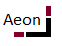
\includegraphics[width=0.2\textwidth]{../Templates/Aeon}\\[1cm] % Include a department/university logo - this will require the graphicx package

	%----------------------------------------------------------------------------------------

	\vfill % Push the date up 1/4 of the remaining page

\end{titlepage}


\section*{\begin{center}Projektidentitet\end{center}}
    \vspace{-2.5em}
    \begin{center}
        \begin{tabular}{|c c c|}
        \hline
        Namn & Roll & E-post \\
        \hline
        Adam Andersson& Teamleader & adam.e.a.andersson@gmail.com\\
        \hline
        Niclas Byrsten & Testansvarig & nicby889@student.liu.se\\
        \hline
        Björn Hvass & Konfigurationsansvarig & bjorn.hvass@gmail.com\\
        \hline
        Henrik Lindström & Utvecklingsledare & henli070@student.liu.se\\
        \hline
        Martin Persson & Arkitekturansvarig & marpe902@liu.student.se\\
        \hline
        Christoffer Sjöbersson & Analysansvarig & chrsj812@liu.student.se\\
        \hline
        Tor Utterborn & Dokument- \& Kvalitetsansvarig & tor.utterborn@gmail.com\\
        \hline
        \end{tabular}
    \end{center}

    \begin{center}
        \small
        \textbf{Kund}\\Region Östergötland, 581 91 Linköping.

        \textbf{Kontaktperson hos kund}\\
        Gunnar Nordqvist, IT-arkitekt, 010-1030698, Gunnar.Nordqvist@regionostergotland.se\\
        Erik Sundvall, Informationsarkitekt, 010-1036252, Erik.Sundvall@regionostergotland.se
    \end{center}

\vspace{9em}



\begin{abstract}
\noindent Vi har under förstudien i iteration två färdigställt ett antal dokument för att definiera vårt projekt. I dessa dokument behandlas ett flertal olika frågeställningar, bakgrund, syfte och mål med projektet. Det finns även dokument där tidsplanen, kraven och milstolparna för projekt har formulerats. Utöver att sammanställa dokumentation har gruppen haft flera utbildningar som har berört bland annat arbetsmetodik och teknisk kompetens.
\end{abstract}
\clearpage

\section{Dokumentation}
\label{sec:Dokumentation}
De dokument som har sammanställts under den första iterationen är följande:

\textbf{Projektplan}\\ Det här dokument innehåller en beskrivning av hur projektet ska genomföras samt varför det ska genomföras.

\textbf{Kravspecifikation}\\ Det här dokumentet behandlar alla krav som är relevanta på produkten som projektet ska resultera i. Dessa krav berör många aspekter bland annat krav på arkitekturen, funktionaliteten och begränsningar.

\textbf{Kvalitetsplan}\\ Den här planen innehåller en form av \emph{hypotes} på hur arbetet i gruppen ska fungera.

\textbf{Systematanomi}\\ Denna anatomi ger en grafisk bild av systemet som ska utvecklas i projektet.

\section{Utbildning och forskning}
\label{sec:Utbildning och forskning}
Under första iterationen har gruppen tagit del av diverse utbildningar för att förbereda inför kommande iterationer.

\textbf{Git}\\ Gruppen har haft en genomgång av git som versionshanteringsverktyg samt featurebranch-workflow. Syftet med den här genomgången var att ge gruppen en introduktion till Git, hur det fungera samt hur gruppen kommer arbeta med det under projektet.

\textbf{Scrum}\\ Gruppen har haft en genomgång av arbetsmetodiken Scrum som används i projektet. Syftet med den här genomgången var att introducera Scrum och hur gruppen kommer att använda sig av det under kursens gång.

\textbf{Seminarium och föreläsningsserie i kursen TDDD96}\\ Gruppen har även tagit del av den officiella utbildningen som erbjuds i kursen TDDD96. Ämnen som här berörts inkluderar:
\begin{itemize}
    \item Hållbar utveckling
    \item Projektarbetet
    \item Dokumentskrivning
    \item Att sälja en idé
    \item Dela kunskap om design
\end{itemize}

\textbf{\LaTeX}\\ Under iterationen tog gruppen ett beslut om att använda LaTeX för att skriva dokument. Som ett resultat av det så har gruppens medlemmar avsatt tid för att sätta sig in LaTeX.

\textbf{Standarder}\\ Eftersom många av dokumenten som skrevs under iterationen följer standarder har gruppen satt sig in i ett flertal olika standarder. Syftet med att göra det är att skaffa kunskap till konstruktionen av mallar för dokumenten som beskrevs i sektion \ref{sec:Dokumentation}.

\section{Kund}
Under iterationen har gruppen haft ett antal möten med kund.

\textbf{Förstamötet}\\
Under det första mötet med kund träffade två representanter från gruppen kunden och gick igenom övergripande information, vilka förväntningar som fanns och vilka resurser som de hade till godo.

\textbf{Uppstartsmöte}\\
Under det här mötet träffade hela gruppen kunden för första gången. Under mötet fick gruppen en presentation som tog upp bakgrund, förväntningar och nuvarande status.

\textbf{Kravmöte}\\
Under kravmötet gick två gruppmedlem igenom kundens kravlista, den listan reviderades under mötets gång och alla fick en klar blid av vad det var som skulle ingå i kraven.

\textbf{Arkitekturmöte}\\
Två av gruppen medlemmar hade ett möte om arkitekturen för projektet. Här fick gruppen flera tips på hur man kunde bygga systemet.

\section{Måluppfyllnad}
Gruppen har uppnått målen för den här iterationen. De uppgifter som planerades att genomföras i den här iterationen har färdigställts i tid utan komplikationer.

\end{document}
